\documentclass[a4,center,fleqn]{NAR}
\usepackage{amsmath} %added by SAM
\usepackage{hyperref} %added by SAM
\usepackage[nodisplayskipstretch]{setspace} %added by SAM 
\setstretch{1.5} %added by SAM
\usepackage{longtable} %added by SAM
\usepackage{comment} %added by SAM
% Enter dates of publication
\copyrightyear{2021}
\pubdate{DD MM YYYY}
\pubyear{YYYY}
\jvolume{xx}
\jissue{xx}

%\articlesubtype{This is the article type (optional)}

\begin{document}

\title{Ribofilio: A tool to estimate ribosomes drop-off rate in Saccharomyces Cerevisiae}

\author{%
Corresponding Author\,$^{1,*}$,
First Co-Author\,$^{2}$
and Second Co-Author\,$^2$%
\footnote{To whom correspondence should be addressed.
Tel: +44 000 0000000; Fax: +44 000 0000000; Email: xxx@yyyy.ac.zz}}

\address{%
$^{1}$Affiliation of Corresponding Author
and
$^{2}$Affiliation of Both Co-Authors}
% Affiliation must include:
% Department name, institution name, full road and district address,
% state, Zip or postal code, country

\history{%
Received YYYY-MM-DD;
Revised YYYY-MM-DD;
Accepted YYYY-MM-DD}

\maketitle

\begin{abstract}
The premature ribosome drop-off phenomenon plays crucial roles in translational accuracy. However, the quantification of ribosome drop-off in Saccharomyces cerevisiae is sill under study.  
We provide `Ribofilio` a python tool that rely on a high sensitive binning strategy to estimate the ribosome drop-off rate in Saccharomyces cerevisiae. We show that a significant rate of ribosome drop-off is both measurable and quantifiable. Moreover, we show that the drop-off rate is variable, depending on stress conditions, gene length, and  gene ontology.  

Ribofilio is available on conda and github: 
\href{url}{https://github.com/SherineAwad/ribofilio.git}. A tutorial to ribosomal profiling protocol usig ribofilio is found here: \href{url}{https://ribofilio.readthedocs.io/en/latest/protocol.html}
\end{abstract}


\section{Introduction}

Translation of messenger RNA (mRNA) into proteins is a complex process. Ribosomes play a pivotal role in ensuring that mRNA is decoded accurately and rapidly.   \cite{keedy2018,ramakrishnan2002}. However, this translation machinery is prone to errors. One of the possible errors occurs when the ribosome fails to complete a full-length synthes process of a protein. This leads to a premature termination of the translation process. \cite{ou2019errors,chiarugi2016}.
There are various mechanisms known to intervene in the translation abortion. Some of these mechanisms exert their strength  when the cell faces stressing conditions that hinder mRNA translation, e.g. amino acid starvation. \cite{yip2021detecting}. 
In bacteria, the tmRNA-SmpB complex \cite{keiler1996role, keiler2015mechanisms}  , RF3  \cite{zaher2011primary} , ArfA \cite{chadani2010ribosome} and ArfB  \cite{chadani2011escherichia} are main abortion-mediating factors known to help rescue stalling ribosomes and eventually lead to premature termination of protein synthesis.
Moreover, a proofreading mechanism interrupts the synthesis of miscoded polypeptides in a translation abandonment process. \cite{zaher2009quality}

There is also the possibility of unspecific events which can interrupt  the elongation of the nascent peptide commonly known as processivity errors. \cite{gilchrist2006, kurland1993, kurland1992}. This includes 
a false stop codon causing a premature termination,  \cite{baranov2015augmented,gurvich2003sequences}. 

In addition, a drop-off of ribosomes can be triggered by , local depletion of ternary complexes. \cite{zhang2010global}

All these translation abandoment factors and processivity errors prevent the ribosome from reaching the final stop codon. 
We will use the term `ribosomes drop-off rate` to denote all the events that entail the premature detachment of the ribosomes from the mRNA template, irrespective of the mechanism  that caused this event. 


Ribosomes drop-off doesn't necessarily occur in stressing conditions.\cite{kurland1992,jorgensen1990processivity}. The frequency of ribosomes drop-off rate is expected  to be at a ‘basal’ value when the cell is not facing any stressing conditions. 



% **************************************************************
% Keep this command to avoid text of first page running into the
% first page footnotes
\enlargethispage{-65.1pt}
% **************************************************************

 

Chiarugi et al. in \cite{chiarugi2016} provides a quantitative method for ribosomes drop-off rate in E.Coli. We are extending their approach in Saccharomyces cerevisiae, and studying the effect of gene length and gene ontology categories on the drop-off rate. 


\section{MATERIALS AND METHODS}


\subsection{Ribofilio: A tool for estimating drop-off rate} 
We developed `ribofilio` an open source  python tool to estimate the drop-off rate of ribosome. Ribofilio is found on our github repository \url{https://github.com/SherineAwad/ribofilio/}.  Ribofilio takes as input the genome transcripts, the footprint reads in bed format and if mRNA reads is provided, ribofilio will normalize the drop-off rate using the mRNA reads.
Ribofilio runs on a full list of genes, a subset of genes, or even on a single gene.
We also provide a tutorial to how to estimate  drop off rate of ribosomes using ribofilio starting from fastq reads: \url{https://ribofilio.readthedocs.io/en/latest/protocol.html} 

A snakemake reproducible pipeline is found in our github repository \url{https://github.com/SherineAwad/ribofilio/pipeline}. All scripts are found in our \url{https://github.com/SherineAwad/ribofilio/pipeline/scripts/}.  In addition, a user can run our pipeline using `\texttt{-{}-}use-conda` mode to pull the same tools' versions we used. 

\subsection{Data Preparation}

We used ten datasets from GSE91068 and GSE134152 from GEO see Table \ref{tab1}. We used trim\_galore to trim adapters and quality filter the reads. We used  trim\_galore's default parameters and -a was set to the corresponding adapters shown in Table 2 supplementary text. We then aligned the reads to yeast transcripts Saccharomyces\_cerevisiae.R64-1-1.cdna.all.fa using bowtie2 \cite{langmead2012fast} and generated a bed file using `bedtools bamtobed` command \cite{quinlan2010bedtools}.  See Table 1 in the supplementary text for the unique alignments percentages for all the datasets. For the sake of reproducibility, we provide a Makefile to pull the datasets  and the yeast genome we used: \url{https://github.com/SherineAwad/ribofilio/tree/master/data/Makefile}.


\subsection{Gene Ontology and Gene Length Subsets} \label{GOGL}

We downloaded the gene ontology from biomart using our script `getGO.R`. We used `gcluster.py` script to cluster genes based on their length: [0-500], ]500-1000], ]1000-2000] , ]2000, 3000], ]3000-4000], ]4000-5000], and ]5000-$\infty$]. All scripts are found in \url{https://github.com/SherineAwad/ribofilio/pipeline/scripts/}.


\subsection{Computing the average number of RPFs per ORF: a binning strategy}
Here we explain the core of ‘ribofilio‘.
For each dataset reported in Table 1, we created a nucleotide
vector positions where position i reports the number of ORFs that their 3’ end is at position i. We normalized each ıin positions vector with the number of genes that their length covers position i.
\begin{equation*} \label{eq:1}
positions_{i}= \frac{total RNAseq reads for ORF_{i}}{Li}
\end{equation*}
where Li is the number of genes which their length reach position i.
Then grouped all positions into bins of size BINSIZE. This results in the Bin vector composed by cells (i):
\begin{equation*} \label{eq:2}
BIN_{(j)} = \frac{\sum_{j}{positions_{i}}} {BINSIZE}
\end{equation*}

We use the RPF reads to generate the RPF Bin vector and similarly use their RNA-seq reads to generate the RNA Bin vector. To normalize the amount of RPFs with the abundance of the corresponding RNA-seq reads, we divided the value in each cell of the RPF Bin vector by their corresponding RNA Bin (i) given by:

\begin{equation*} \label{eq:3}
    NRPF_{(i)} = \frac{RPF_{i}}{RNA_{i}}
\end{equation*}



\subsection{Estimation of Drop-off rate and its standard error}

\begin{equation*} \label{eq:4}
Y=A∗e^{-RX}
\end{equation*}

We estimate the relationship between average number of RPFs per bin Y normalized by its corresponding RNA and the bin number X to obtain an estimation of the drop-off rate r per codon. Following similar theoretical considerations as in XXX, we tested a hypothesis that the dependence of Y on X follows an exponential decay as in equation \eqref{eq:4}

where X is the bin number =1,2, .. and A is the intercept which has no interest in this scope, and R represents the drop-off

rate is the probability per bin that a ribosome prematurely detaches from the mRNA template. The drop-off rate per codon r reflects that the drop-off rate can occur anywhere inside each bin. Consider r the drop-off rate per codon, then the probability that the ribosome does not drop off within a bin of lc codon is $(1-r)^{lc}$. 
Hence, the probability that the ribosome drop-off rate R drops off anywhere within the bin is $1-(1-r)^{lc} $ and the drop-off per codon r is $1-(1-R)^{lc}$.



 
\begin{table*}[h]
\tableparts{%
\caption{Datasets Description. Column 1 is Dataset ID. Column 2 is GSE series ID. Column 3 is the GSM ID of the footprint. Column 4 is the GSM ID of the corresponding mRNA. Column 5 is Condition details about the dataset. }
\label{tab1}%
}{%
\begin{tabular}{|l|l|l|l|l|}
\hline
Dataset&Series&Footprint & mRNA  & Details 
\\
\hline
D1&GSE91068&
GSM2420488 
&GSM2420486
&Synthetic Defined \\
\hline
D2&GSE134152&(GSM3938053
GSM3938054)
&GSM3938051
&Synthetic Defined (protocol 1) \\
\hline
D3&GSE134152&GSM39380599&GSM3938057
&Synthetic Defined (protocol 2) \\
\hline
D4&GSE91068&GSM2420489&GSM2420487
&Methionine Restriction \\
\hline
D5&GSE134152&(GSM3938055,
GSM3938056)
&GSM3938052 
&Glucose Restriction (protocol 1) \\
\hline
D6&GSE134152&GSM3938060&GSM3938058
&Glucose Restriction (protocol 2) \\
\hline
D7&GSE13750&GSM346111&GSM346117&Rich  (1)	\\ 
\hline
D8&GSE13750&GSM346114&GSM346118&Rich (2) \\
\hline
D9&GSE13750&GSM346115&GSM346120&Starved (1) \\
\hline
D10&GSE13750&GSM346116&GSM346122&Starved (2)\\
\hline
\end{tabular}%
}

\end{table*}


\begin{table*}[t]
\tableparts{%
\caption{Drop-off rate for Control datasets D1, D2, and D3. Column 1: Dataset  ID  (see  Table \ref{tab1} for a description of each dataset). Column 2: Drop-off rate (R). Column 3: Drop-off rate per codon (r). Column 4: RMSE. Column 6: R square Column 7: Standard Error Estimate (SE).Column 8: Confidence Interval 95\%. Column 9: Pvalue: Null Hypothesis that the drop-off rate is not different from a slope of zero}
\label{tab2}%
}{%
\begin{tabular} {|l|l|l|l|l|l|l|l|}
\hline
Dataset &Drop-off (R) & drop-off per codon (r)&RMSE& Rsquare&SE&CI &Pvalue\\
\hline
D1&-0.0051& -0.0003& 0.0143 & 0.4907 & 0.0006&R$\pm$0.0011&\textless 0.00001  \\
\hline
D2&0.004  & 0.0002&  0.0298&  0.2231&  0.0003 &R$\pm$0.0006& \textless 0.00001 \\
\hline
D3&-0.0102 &-0.0006 &0.025&   0.6887&  0.0007 &R$\pm$0.0013&\textless 0.00001 \\
\hline
\end{tabular}%
}

\end{table*}




\begin{table*}[t]
\tableparts{%
\caption{Drop-off rate for Treatment datasets D4, D5, and D6. Column 1: Dataset  ID  (see  Table \ref{tab1} for a description of each dataset). Column 2: Drop-off rate (R). Column 3: Drop-off rate per codon (r). Column 4: RMSE. Column 6: R square Column 7: Standard Error Estimate (SE).Column 8: Confidence Interval 95\%. Column 9: Pvalue: Null Hypothesis that the drop-off rate is not different from a slope of zero}
\label{tab3}%
}{%
\begin{tabular} {|l|l|l|l|l|l|l|l|}
\hline
Dataset &Drop-off (R) & drop-off per codon (r)&RMSE& Rsquare&SE&CI &Pvalue\\
\hline
D4&-0.01 &-0.0006& 0.0762 & 0.4104&  0.0011 &R$\pm$0.0021  & \textless 0.00001   \\
\hline
D5&0.0004 & 0.0  &   0.1127&  0.0007&  0.0003 &R$\pm$0.0007  &0.133   \\
\hline
D6&-0.0073 &-0.0004& 0.0282  &0.4993&  0.0003 &R$\pm$0.0006  &\textless 0.00001  \\
\hline
\end{tabular}%
}

\end{table*}



\begin{table*}[t]
\tableparts{%
\caption{Drop-off rate per codon for Treatment datasets D7, D8, D9, and D10. Column 1: Dataset  ID  (see  Table \ref{tab1} for a description of each dataset). Column 2: Drop-off rate (R). Column 3: Drop-off rate per codon (r). Column 4: RMSE. Column 6: R square Column 7: Standard Error Estimate (SE).Column 8: Confidence Interval 95\%. Column 9: Pvalue: Null Hypothesis that the drop-off rate is not different from a slope of zero}
\label{tab4}%
}{%
\begin{tabular} {|l|l|l|l|l|l|l|l|}
\hline
Dataset &Drop-off (R) & drop-off per codon (r)&RMSE& Rsquare&SE&CI &Pvalue\\
\hline
D7&-0.0057& -0.0003& 0.4843 & 0.0341& 0.0021&R$\pm$0.0041&0.0038  \\
\hline
D8&-0.0053& -0.0003 &0.3147&  0.0462 & 0.0019  &R$\pm$0.0038  &0.0029     \\
\hline
D9&-0.0079 &-0.0005& 0.5336&  0.0594 & 0.0027 & R$\pm$0.0053  &0.0016   \\
\hline
D10& -0.0077& -0.0005& 0.4188&  0.0709 & 0.0027 &R$\pm$ 0.0052  & 0.002   \\
\hline
\end{tabular}%
}

\end{table*}



\begin{table*}[t]
\tableparts{%
\caption{Drop-off rate per codon for dataset D1 per GO subsets: Column 1: GO ID  (see Supplementary Table 01 for the respective GO names). Column 2: Drop-off rate (R). Column 3: Drop-off rate per codon (r). Column 4: RMSE. Column 6: R square Column 7: Standard Error Estimate (SE).Column 8: Confidence Interval 95\%. Column 9: Pvalue: Null Hypothesis that the drop-off rate is not different from a slope of zero}
\label{tab5}%
}{%
\begin{tabular} {|l| p{0.3cm}|l|l|l|l|l|l|l|l|}
\hline
\multicolumn{10}{|c|}{D1} \\
\hline
GO&Size&Description&Drop-off (R) & drop-off per codon (r)&RMSE& Rsquare&SE&CI &Pvalue\\
\hline
GO:0006950&33& Response to Stress&-0.2064&-0.0113&3.2499&0.7287&0.021&R$\pm$0.0418&\textless 0.00001\\
\hline
GO:0022857&111&Transmembrane Transporter Activity&-0.04&-0.0024&0.0601&0.7682&0.0042&R$\pm$0.0084&\textless 0.00001\\
\hline
\multicolumn{10}{|c|}{D2} \\
\hline
GO:0006950&33&Response to Stress&-0.2265&-0.0123&3.5607 &0.7471&0.0207&0.0412&\textless 0.00001\\
\hline
\multicolumn{10}{|c|}{D3} \\
\hline
GO:0006950&33&Response to Stress&-0.2166&-0.0118&4.4808&0.6821&0.0241&R$\pm$0.0482&\textless 0.00001\\
\hline
GO:0022857&111&Transmembrane Transporter Activity&-0.0568&-0.0033&0.0888&0.8188&0.009&R$\pm$0.018&\textless 0.00001\\
\hline
GO:0030684&2&Preribosome&-0.0594&-0.0035&0.0909&0.6985&0.0078&R$\pm$0.016& \textless 0.00001\\
\hline
GO:0044249&6&Cellular biosynthetic process&-0.0747& -0.0043& 0.0864&  0.7758&  0.008& R$\pm$ 0.0164  & \textless 0.00001 \\
\hline
GO:0009651&20&Response to Salt Stress &-0.0467&-0.0027&0.2279&0.7495&0.0035&R$\pm$0.0069&\textless 0.00001\\
\hline
\end{tabular}%
}

\end{table*}

\begin{table*}[t]
\tableparts{%
\caption{Drop-off rate per codon for dataset D1 and dataset D3 per Gene Length subsets: Column 1: Gene Length sub-group. Column 2: Drop-off rate (R). Column 3: Drop-off rate per codon (r). Column 4: RMSE. Column 5: Standard Error Estimate (SE).Column 6: Confidence Interval 95\%. Column 7: Pvalue: Null Hypothesis that the drop-off rate is not different from  a slope of zero}
\label{tab6}%
}{%
\begin{tabular} {|l|l|l|l|l|l|l|l|}
\hline
\multicolumn{7}{|c|}{D1} \\
\hline
Gene Length&Drop-off (R) & drop-off per codon (r)&RMSE & Rsquare& SE&CI &Pvalue\\
\hline
$<$500&0.0275&0.0017&0.0628&0.0663&0.0362&R$\pm$0.0834 &0.2341 \\
\hline
]500-1000]&-0.0607&-0.0035&0.0454&0.6601&0.0111&R$\pm$0.0234&\textless 0.00001 \\
\hline
]1000-2000]&-0.0375&-0.0022&0.0356&0.7754&0.0031&R$\pm$0.0063&\textless 0.00001 \\
\hline
]2000-3000]&-0.0281&-0.0017&0.0302&0.8478&0.0013&R$\pm$0.0026&\textless 0.00001 \\
\hline
]3000-4000]&-0.0265&-0.0016&0.0249&0.9196&0.0008&R$\pm$0.0016&\textless 0.00001 \\
\hline
]4000-5000]&-0.0228&-0.0014&0.0354&0.9088&0.0007&R$\pm$0.0014 &\textless 0.00001 \\
\hline
$>$5000&-0.0133&-0.0008&0.0784&0.8355&0.0007 &R$\pm$0.0013&\textless 0.00001 \\
\hline
\multicolumn{7}{|c|}{D2} \\
\hline
Gene Length&Drop-off (R) & drop-off per codon (r)&RMSE& Rsquare &SE&CI &Pvalue\\
\hline
$<$500&-0.0409& -0.0024& 0.175&   0.0531&  0.0452 &R$\pm$0.1043 &0.1964  \\
\hline
]500-1000]& -0.0284& -0.0017& 0.0186&  0.5091&  0.0089&R$\pm$0.0187& 0.0025 \\
\hline
]1000-2000]& -0.02  & -0.0012 &0.0151  &0.6989  &0.0019  &R$\pm$0.0039&\textless 0.00001  \\
\hline
]2000-3000]&-0.019 & -0.0011 &0.0097 & 0.8873 & 0.0009&R$\pm$0.0018&\textless 0.00001  \\
\hline
]3000-4000]&-0.019 & -0.0011 &0.0127 & 0.92  &  0.0007&R$\pm$0.0013& \textless 0.00001  \\
\hline
]4000-5000]&-0.0179& -0.0011& 0.0363&  0.8568 & 0.0007&R$\pm$0.0014&\textless 0.00001  \\
\hline
$>$5000&-0.0093 &-0.0006 &0.0488 & 0.7989 & 0.0005 &R$\pm$0.0009&\textless 0.00001  \\
\hline
\multicolumn{7}{|c|}{D3} \\
\hline
Gene Length&Drop-off (R) & drop-off per codon (r)&RMSE& Rsquare &SE&CI &Pvalue\\
\hline
$<$500&-0.0304&-0.0018&0.0586&0.0846&0.0274&R$\pm$0.0631&0.1499 \\
\hline
]500-1000]&-0.1104&-0.0063&0.0272&0.9144&0.007&R$\pm$0.0147&\textless 0.00001 \\
\hline
]1000-2000]&-0.0589&-0.0034&0.0368&0.8914&0.0032&R$\pm$0.0065&\textless 0.00001 \\
\hline
]2000-3000]&-0.0378&-0.0022&0.0402&0.8831&0.0016&R$\pm$0.0031&\textless 0.00001 \\
\hline
]3000-4000]&-0.0328&-0.0019&0.0436&0.9089&0.0011&R$\pm$0.0023&\textless 0.00001 \\
\hline
]4000-5000]&-0.0268&-0.0016&0.0477&0.9113&0.0009&R$\pm$0.0017&\textless 0.00001 \\
\hline
$>$5000&-0.0139&-0.0008&0.0818&0.8407&0.0006&R$\pm$0.0012&\textless 0.00001 \\
\hline
\end{tabular}%
}

\end{table*}

\begin{figure*} [ht]
\centering
\begin{tabular}{ll}
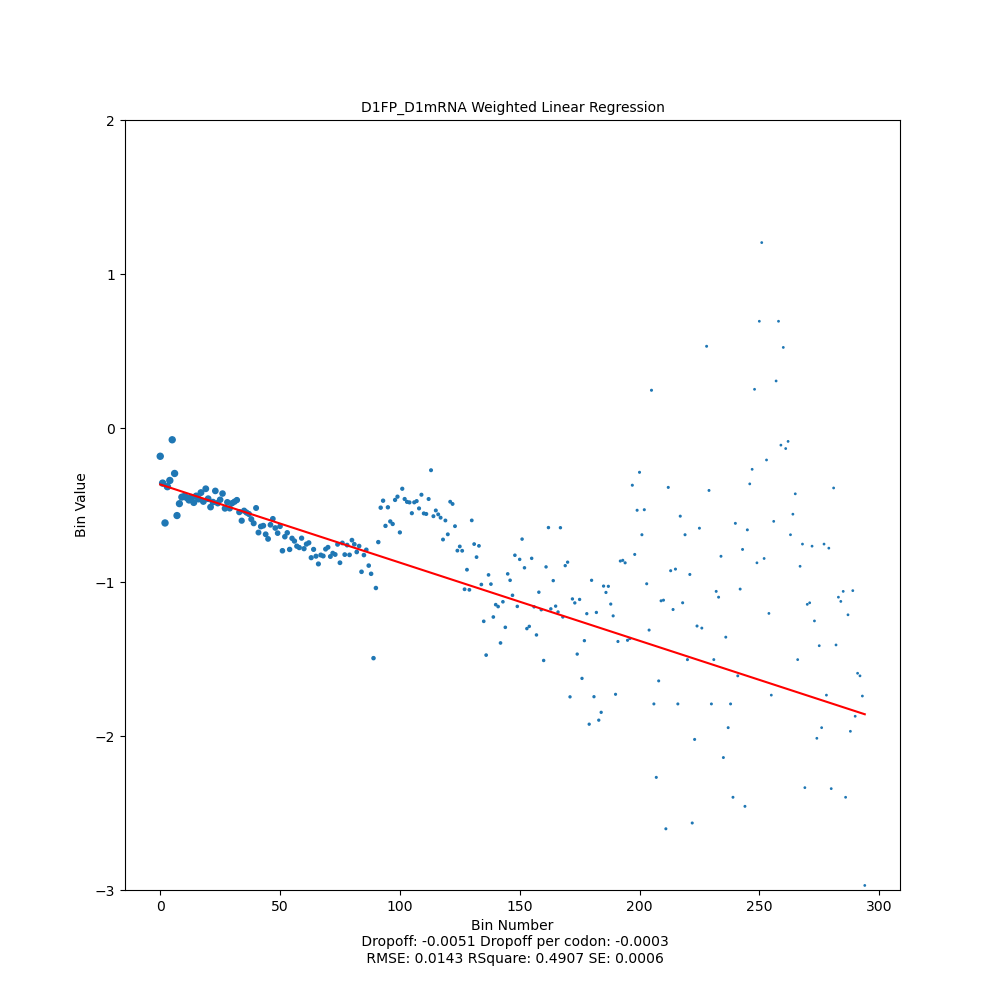
\includegraphics[width=9cm,height=9cm]{D1FP_D1mRNA.Log.WLR.png} & 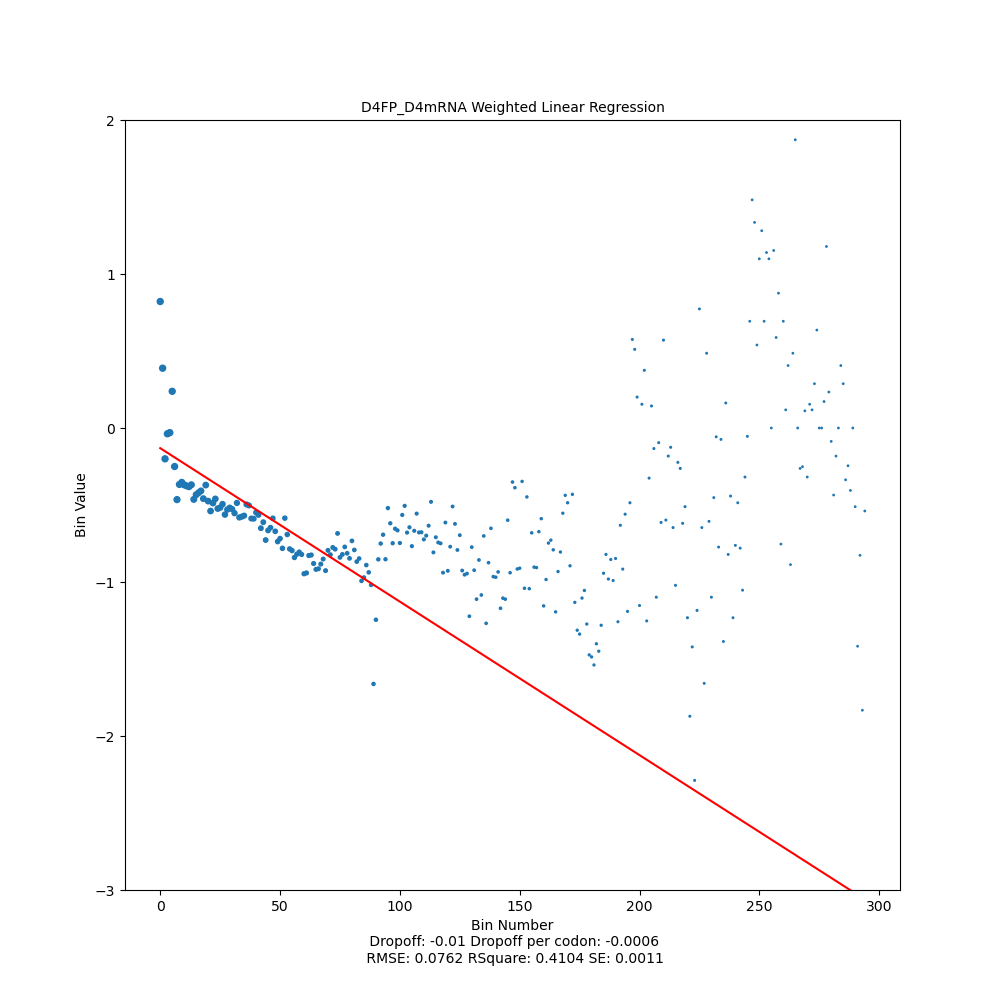
\includegraphics[width=9cm,height=9cm]{D4FP_D4mRNA.Log.WLR.png} \\
\textbf{(a)}   & \textbf{(b)}     \\[0.1pt]
\end{tabular}
\caption{Weighted Linear Regression plot for vector NRPF for control dataset D1 and its corresponding treatment condition dataset D4. The x-axis is the bin number and the y-axis is the vector NRPF in Log exponential. The red line corresponds to the drop-off rate r.
\textbf{(a)} D1 
\textbf{(b)} D4
}
\label{fig1}
\end{figure*}

\begin{figure*} [ht]
\centering
\begin{tabular}{ll}
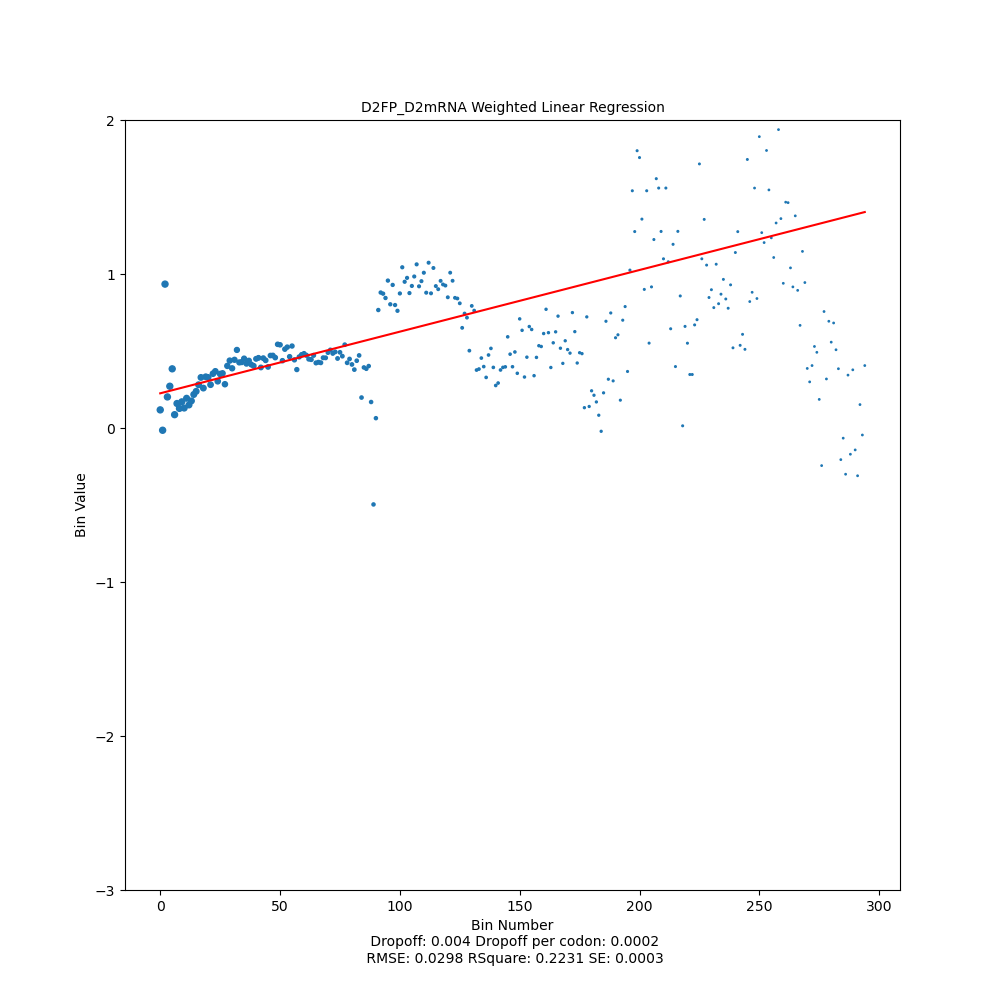
\includegraphics[width=9cm,height=9cm]{D2FP_D2mRNA.Log.WLR.png} & 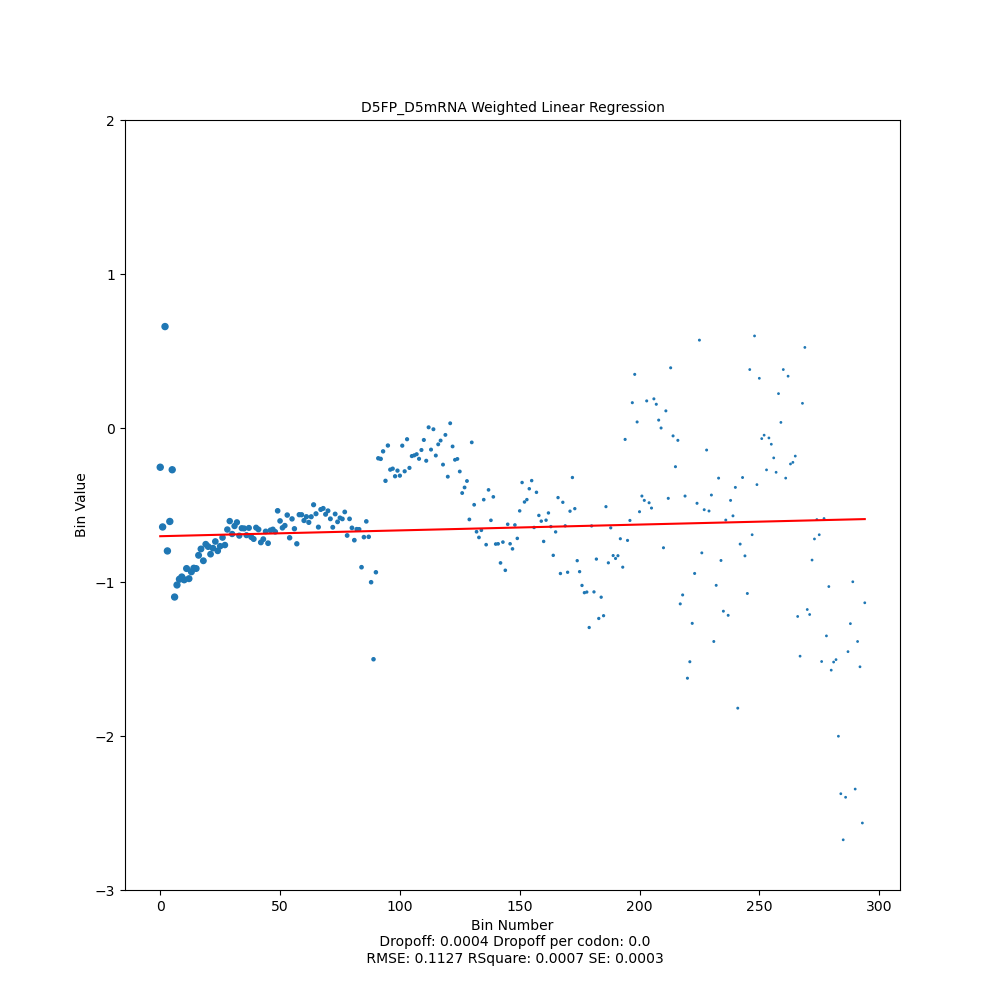
\includegraphics[width=9cm,height=9cm]{D5FP_D5mRNA.Log.WLR.png} \\
\textbf{(a)}   & \textbf{(b)}     \\[0.1pt]
\end{tabular}
\caption{Weighted Linear Regression plot for vector NRPF for control dataset D2 and its corresponding treatment condition dataset D5. The x-axis is the bin number and the y-axis is the vector NRPF in Log exponential. The red line corresponds to the drop-off rate r.
\textbf{(a)} D2
\textbf{(b)} D5
}
\label{fig2}
\end{figure*}


\begin{figure*} [ht]
\centering
\begin{tabular}{ll}
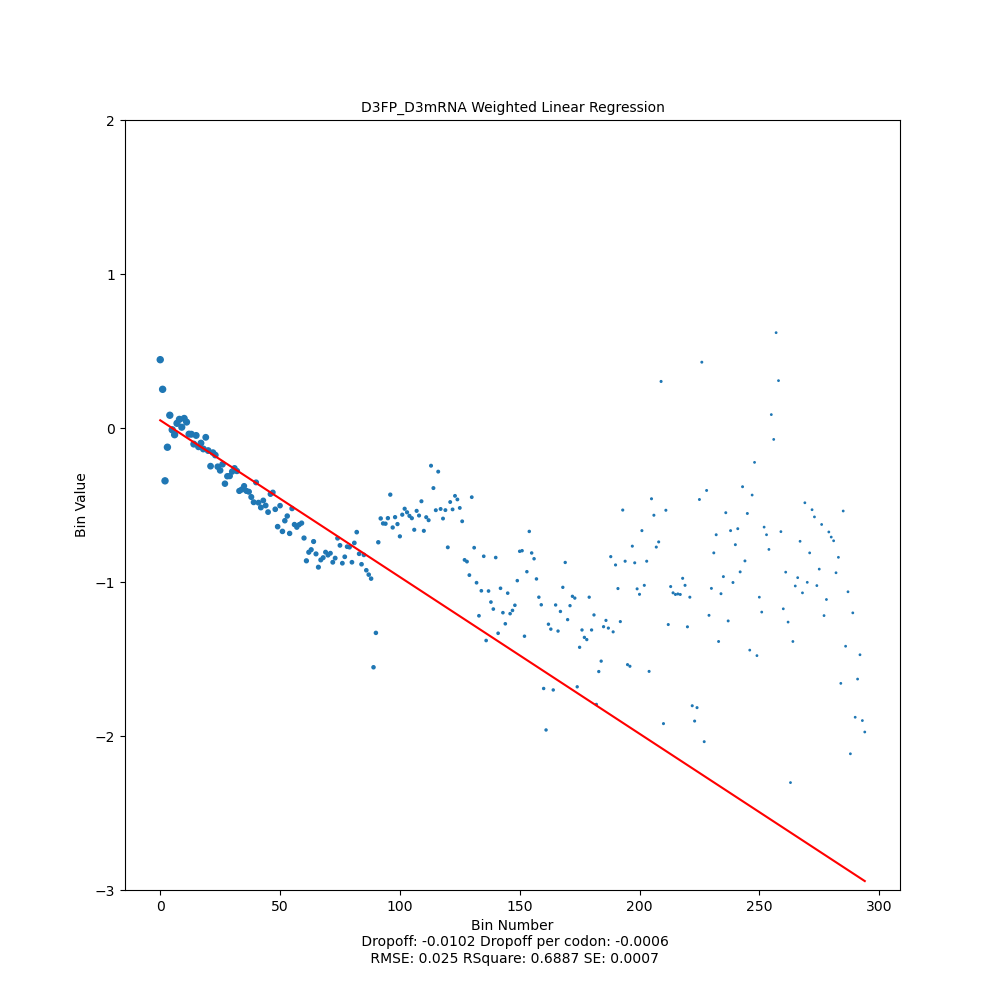
\includegraphics[width=9cm,height=9cm]{D3FP_D3mRNA.Log.WLR.png} & 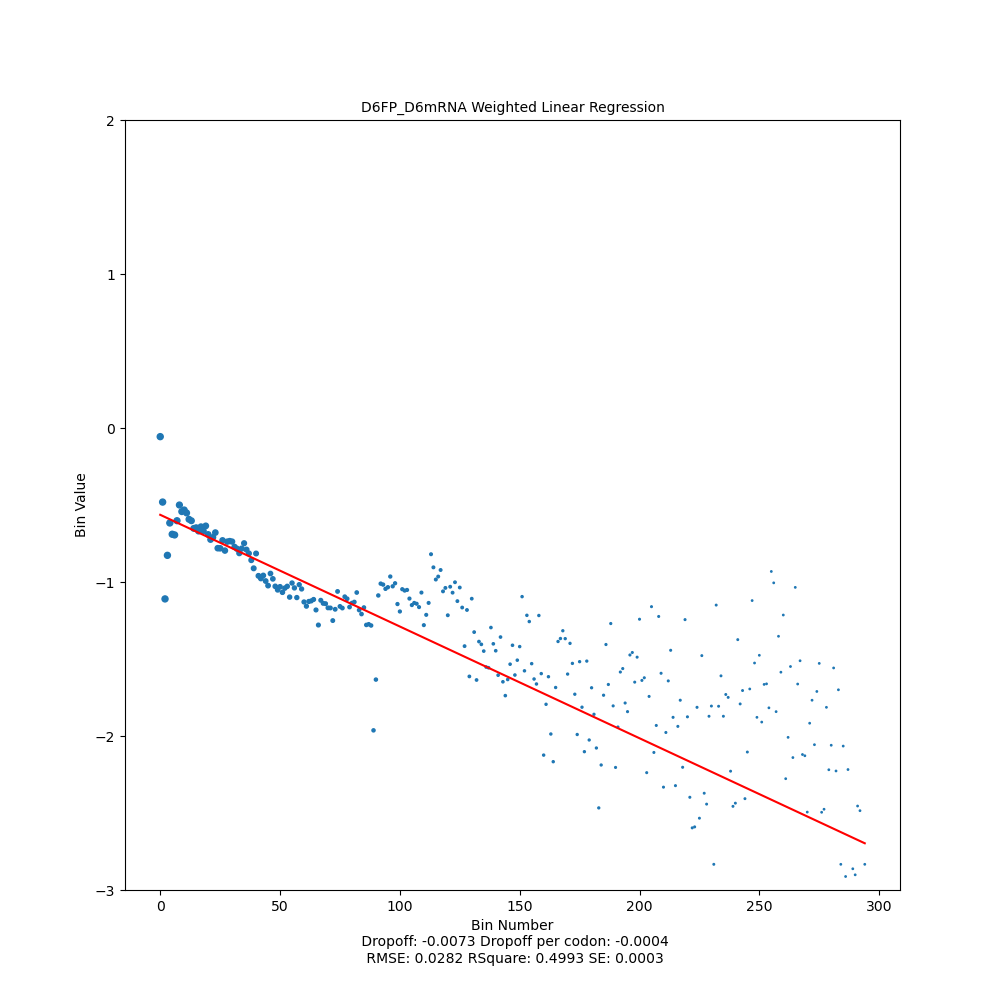
\includegraphics[width=9cm,height=9cm]{D6FP_D6mRNA.Log.WLR.png} \\
\textbf{(a)}   & \textbf{(b)}     \\[0.1pt]
\end{tabular}
\caption{Weighted Linear Regression plot for vector NRPF for control dataset D3 and its corresponding treatment condition dataset D6. The x-axis is the bin number and the y-axis is the vector NRPF in Log exponential. The red line corresponds to the drop-off rate r.
\textbf{(a)} D3
\textbf{(b)} D6
}
\label{fig3}
\end{figure*} 
 

\begin{figure*} [ht]
\centering
\begin{tabular}{ll}
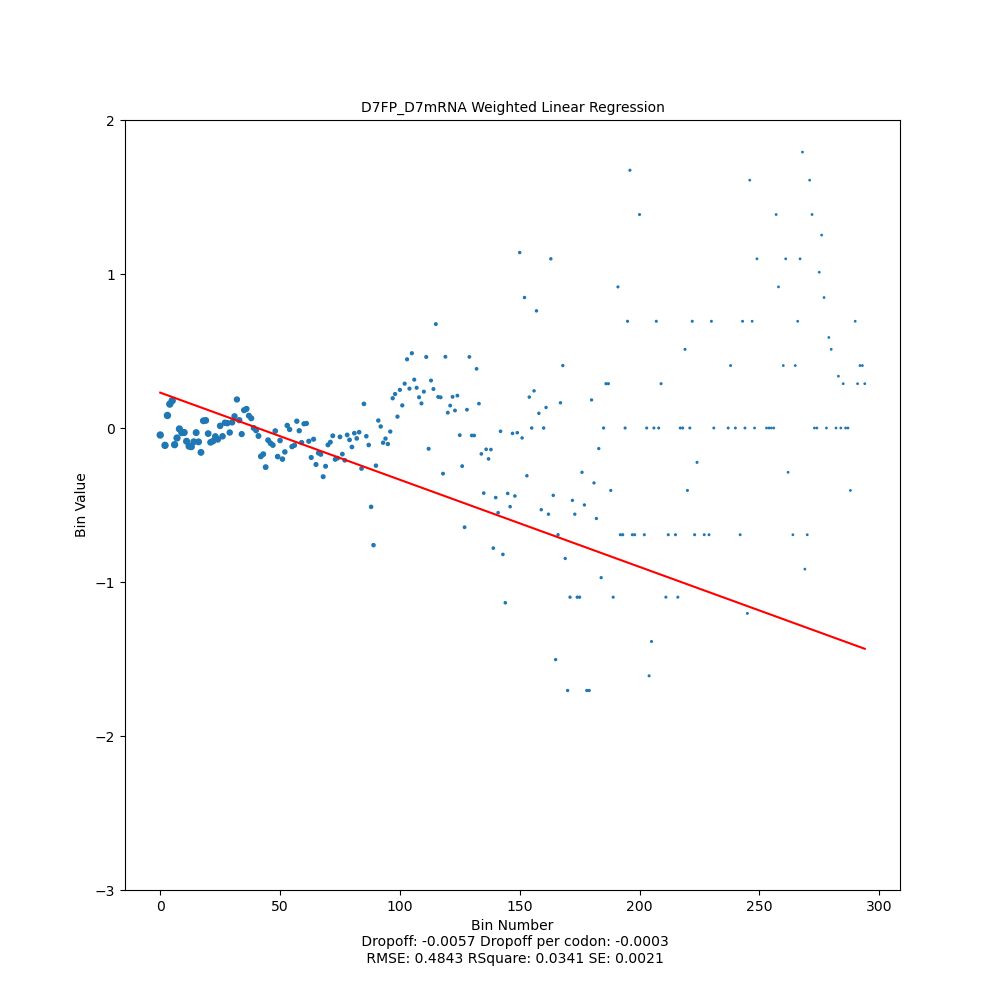
\includegraphics[width=9cm,height=9cm]{D7FP_D7mRNA.Log.WLR.png} & 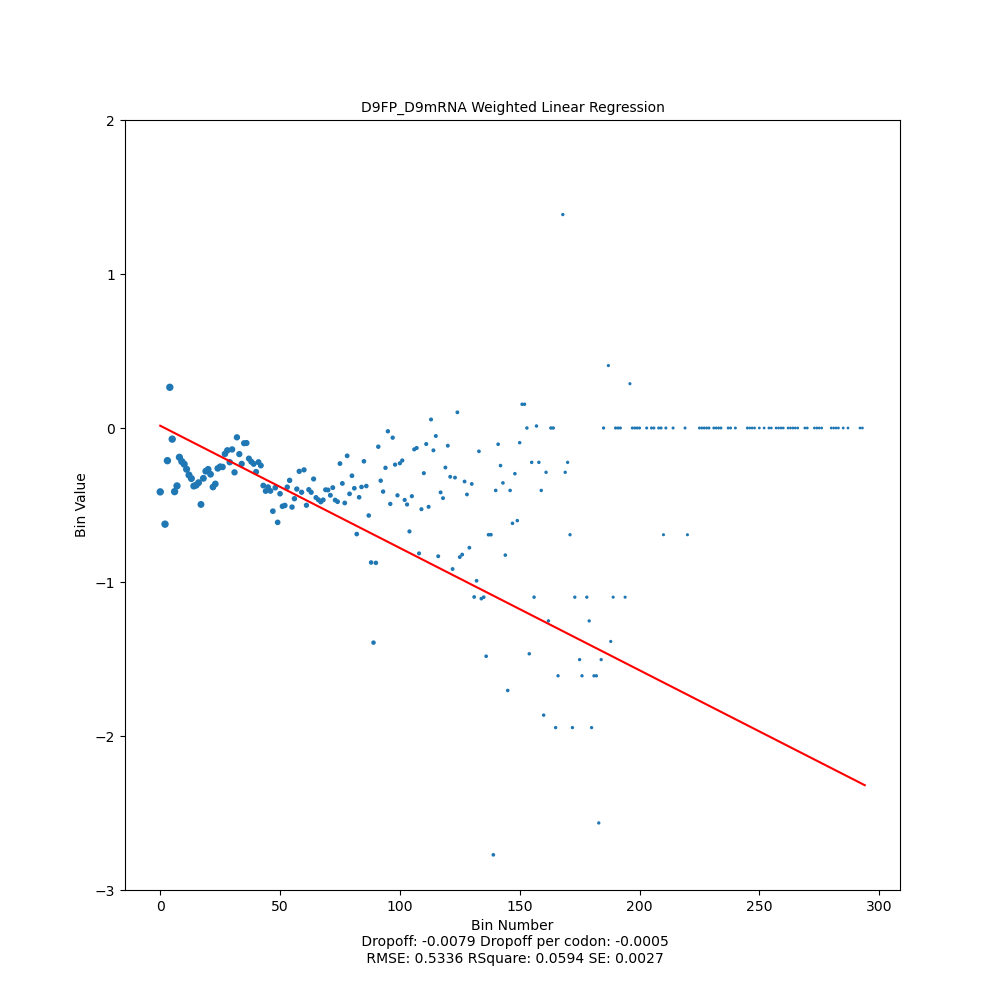
\includegraphics[width=9cm,height=9cm]{D9FP_D9mRNA.Log.WLR.png} \\
\textbf{(a)}   & \textbf{(b)}     \\[0.1pt]
\end{tabular}
\caption{Weighted Linear Regression plot for vector NRPF for rich (1)  dataset D7 and its corresponding starved (1) condition dataset D9. The x-axis is the bin number and the y-axis is the vector NRPF in Log exponential. The red line corresponds to the drop-off rate r.
\textbf{(a)} D7
\textbf{(b)} D9
}
\label{fig4}
\end{figure*} 


\begin{figure*} [ht]
\centering
\begin{tabular}{ll}
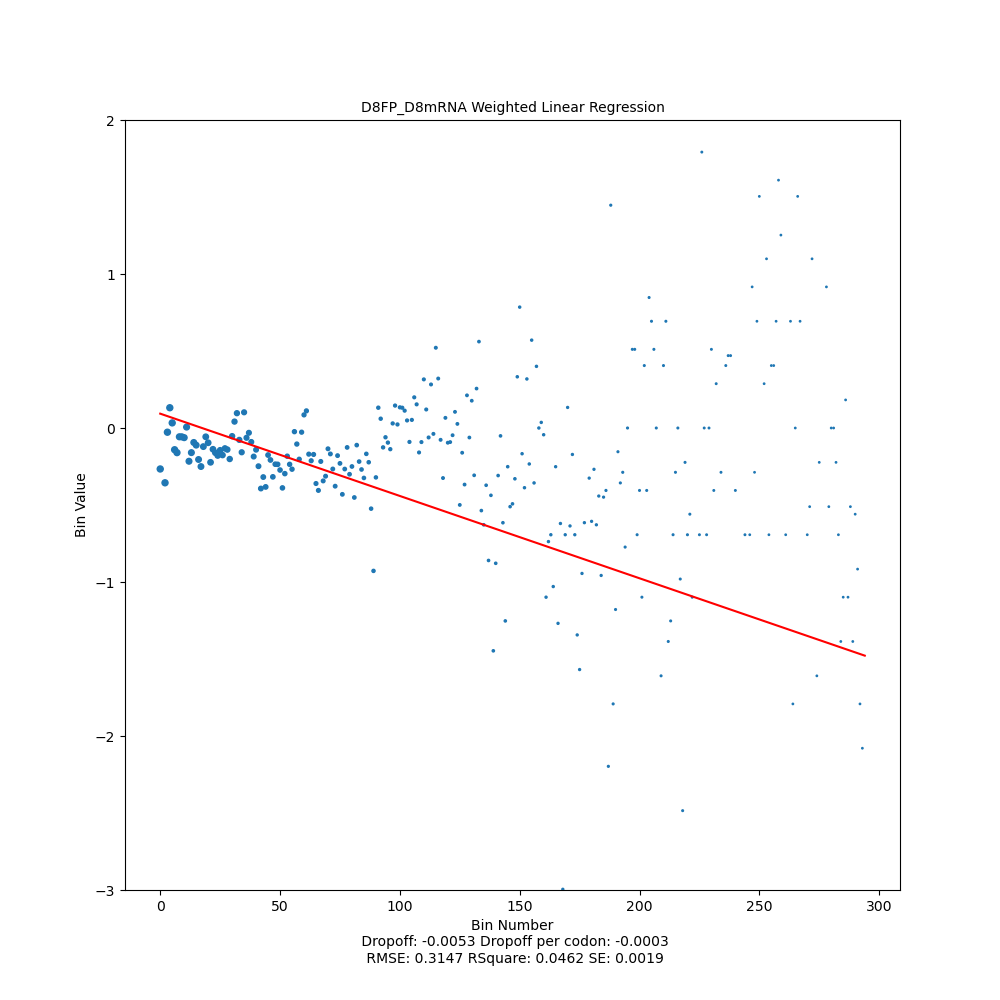
\includegraphics[width=9cm,height=9cm]{D8FP_D8mRNA.Log.WLR.png} & 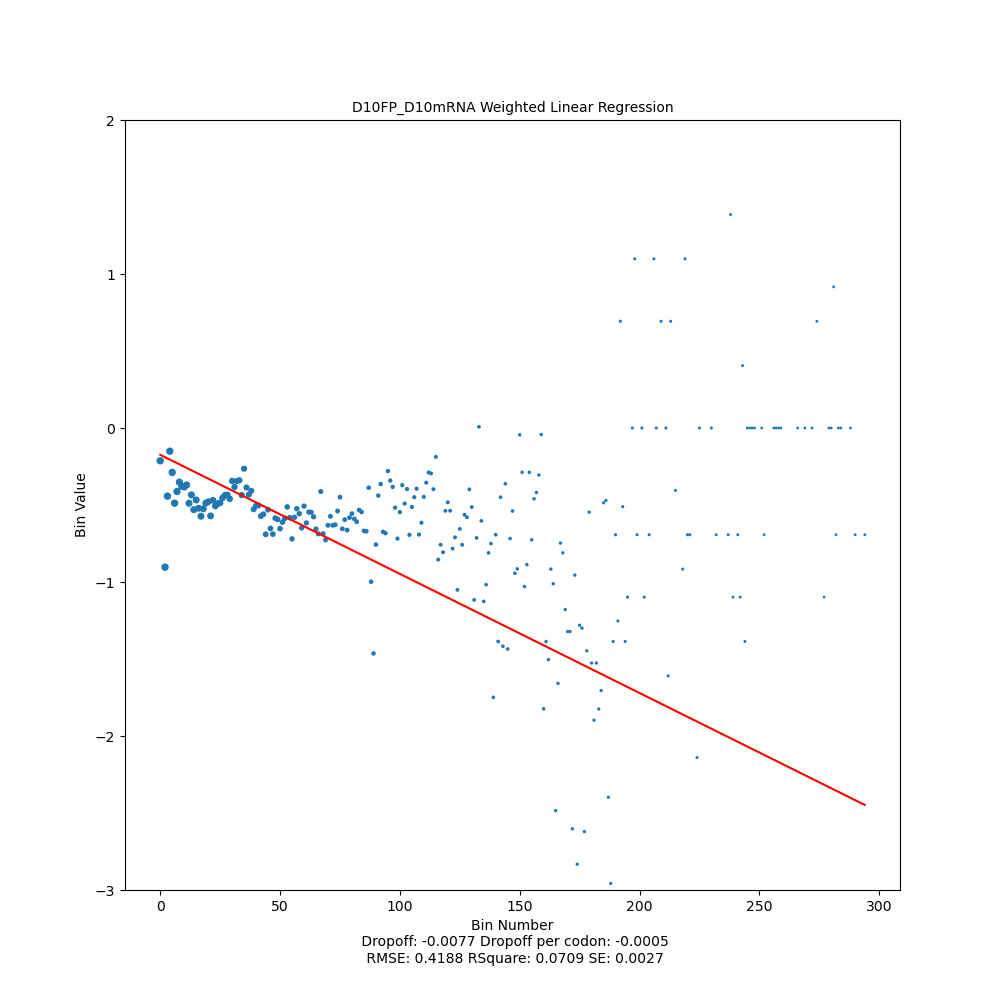
\includegraphics[width=9cm,height=9cm]{D10FP_D10mRNA.Log.WLR.png} \\
\textbf{(a)}   & \textbf{(b)}     \\[0.1pt]
\end{tabular}
\caption{Weighted Linear Regression plot for vector NRPF for rich (1)  dataset D8 and its corresponding starved (1) condition dataset D10. The x-axis is the bin number and the y-axis is the vector NRPF in Log exponential. The red line corresponds to the drop-off rate r.
\textbf{(a)} D8
\textbf{(b)} D10
}
\label{fig5}
\end{figure*} 


\section{Results}
We examined the drop-off rate of three control datasets D1, D2, and D3. See Table \ref{tab2} and Figure \ref{fig1} (a), Figure \ref{fig2} (a), and Figure \ref{fig3} (a) for the drop-off rates of datasets D1, D2, and D3 respectively. The three control datasets show a straight line slope  with RMSE \textless 0.05 with a pvalue \textless 0.01.  This validates our hypothesis that ribosomes drop off at an  exponential decay rate. However, the regression fits introduces some noise reflected by a low Rsquare \textless 70 for the three control datasets. Hence, there could be hidden factors affecting the drop-off rate. To examine these possible factors, we investigated the effect of environmental conditions, gene ontology, and genes length on the drop-off rate. 

\subsection{Drop-off rate is variable based on environmental conditions} 

To examine any possible factor that affect drop-off rate, we studied the drop-off rate of treatment datasets (D4, D5, and D6) of the control datasets (D1, D2, and D3).   The RMSE is \textless 0.5 for D4, D5, and D6, the low Rsquare \textless 70 (see Table \ref{tab3}).  
To examine  whether the treatment condition changes the drop-off rate, we compared the drop-off rate of the control dataset and its corresponding treatment dataset. Table 3 in the Supplementary test shows the drop-off rate and the corresponding fitting statistics of treatment datasets D4, D5, and D6 when compared to the control datasets D1, D2, and D3 respectively. 
Although there is a significant change of the drop-off rate under the treatment condition (see Table 3 Supplementary text),  however, this effect is not the main factor affecting the drop-off rate (See  \ref{tab3}). 

We also examined the drop-off of yeast under both rich and starvation conditions. Table \ref{tab4} shows the drop-off rate for under rich conditions (datasets D7, and D8) and under starvation conditions (datasets D9 and D10). Table 4 in the supplementary text shows  there is no significant change in drop off rate between drop-off rate under rich conditions (D7 and D8) and under starved conditions (D9 and D10). 
Although the RMSE for D7, D8, D9, and D10 are low, the low Rsquare shows that there are other factors affecting the drop off rate rather than the rich and starvation conditions. (See table \ref{tab4}). 


\subsection{Drop-off rate is variable based on gene ontology category}
To further investigate the possible factors that affect the drop-off rate, we run `ribofilio` using subset mode `-s` on different gene ontology terms. See subsection Gene Ontology and Gene Length Subsets \ref{GOGL} and see Table 5 in the supplementary text for the details of each GO category description and set size. 

Table \ref{tab5} shows the significant GO term per each control dataset provided that the GO term shows 1) a significant pvalue \textless 0.01; 2)  a significant  pvalue \textless 0.01 when compared to its corresponding control dataset. 3) Rsquare \textgreater 68\%;  and 4) RMSE \textless 5. 
See Table 6, 7, and 8 in supplementary text for all GO ontology drop-off rate and regression fitting statistics for D1, D2, and D3. See Table 11, 12, and 13 in the supplementary text for a significance t-test comparison between each GO subgroup and its corresponding control dataset. 

The response to stress GO (GO:0006950) with set size equals 33 is commonly significant among the three control datasets D1, D2, and D3.  This shows that although some GO term could affect the drop-off rate of ribosomes, we still need to further investigate other possible factors that affect the drop-off rate of ribosomes.

\subsection{Gene Length affects drop-off rate}

To examine whether gene length could affect the drop-off rate, we run `ribofilio` using subset mode `-s` on different gene length windows (\textless 500, ]500, 1000], ]1000, 2000], ]2000, 3000], ]3000, 4000], ]4000, 5000], and \textgreater 5000). See subsection Gene Ontology and Gene Length Subsets \ref{GOGL}.  Table \ref{tab6} shows the detailed values of drop-off rate, drop-off rate per codon and their corresponding regression fittings for different gene lengths.  We notice that the drop-off rate is decreasing as the gene length increase.

For all control datasets,  and for gene lengths \textgreater 500, the drop-off rate has  Rsquare \textgreater 68 and  RMSE is \textless 0.5. This shows the drop-off rate for gene lengths \textgreater 500 has a very good straight line fit. This indicates not only the drop-off rate follows an exponential decay, but also the drop-off rate for gene length \textgreater 500 don't have the noise previously introduced. 

Also, for all control datasets, D1, D2, and D3, the drop-off rate of gene length greater than 500, the drop-off rate has a significant pvalue \textless 0.01 when compared to a slope of zero. 

Table 14 in the supplementary test shows  the  significance stats of gene length subsets  drop-off rate when compared to the control datasets D1, D2, and D3. The drop-off rate of all gene lengths \textgreater 500 has a significant pvalue \textless 0.01 when compared to the control datasets.  

This shows that the gene length is a significant factor that affect the ribosomes' drop-off rate. 


\begin{comment} to be added later: Tables 9  and 10 in supplementary text show the drop-off rate stats for D4, D5, and D6, and D7, D8, D9, and D10 respectively. The drop-off rate of gene length less than 500 has a pvalue \textgreater 0.1 when compared to a slope of zero for all  datasets  D6, D7, D8, D9, and D10. D4 and D5 has pvalue \textgreater than 0.05 and \textgreater than 0.02. 
Starting from gene length greater than 500, the drop-off rate has a significant pvalue \textless 0.01 when compared to a slope of zero for all  datasets D4, D5, D6, D7, D8, D9, and D10. The drop-off rate is decreasing as the gene length increase. We also compared the significance of a subset of genes clustered by gene length with respect to their main group. Table 14 in the supplementary text shows subsets of gene length greater than 500 are significant with pvalue \textless 0.01 when compared to their main group. 
\end{comment}

\subsubsection{Gene Length affects drop-off rate on control vs treatment datasets}



Table 18 in supplementary text shows the effect of gene length on drop-off rate of control dataset vs their corresponding treatment conditions. 

\section{DISCUSSION AND CONCLUSION}


The ribosome drop-off rate is measurable and quantifiable. Our method is robust against the binsize choice. We have changed the binsize from 25, 50, and 100. The drop-off per rate per codon is constant.  
We have shown that the magnitude of ribosome drop-off is highly variable and dependent on case-specific factors, including experimental conditions  and specific gene ontology categories. 
Furthermore, the drop-off rate increases as the gene length increases. The drop-off rate is close to random when gene length is less than 500. We can conclude that the gene length is a main factor affecting the drop-off rate.  



\clearpage

\section{ACKNOWLEDGEMENTS}
\subsubsection{Conflict of interest statement.} None declared.
\bibliographystyle{plain}
\bibliography{references.bib}

\end{document}
